%
% schwarz.tex -- Gegenbeispiel zum Satz von Schwarz
%
% (c) 2024 Prof Dr Andreas Müller
%
\begin{figure}
\centering
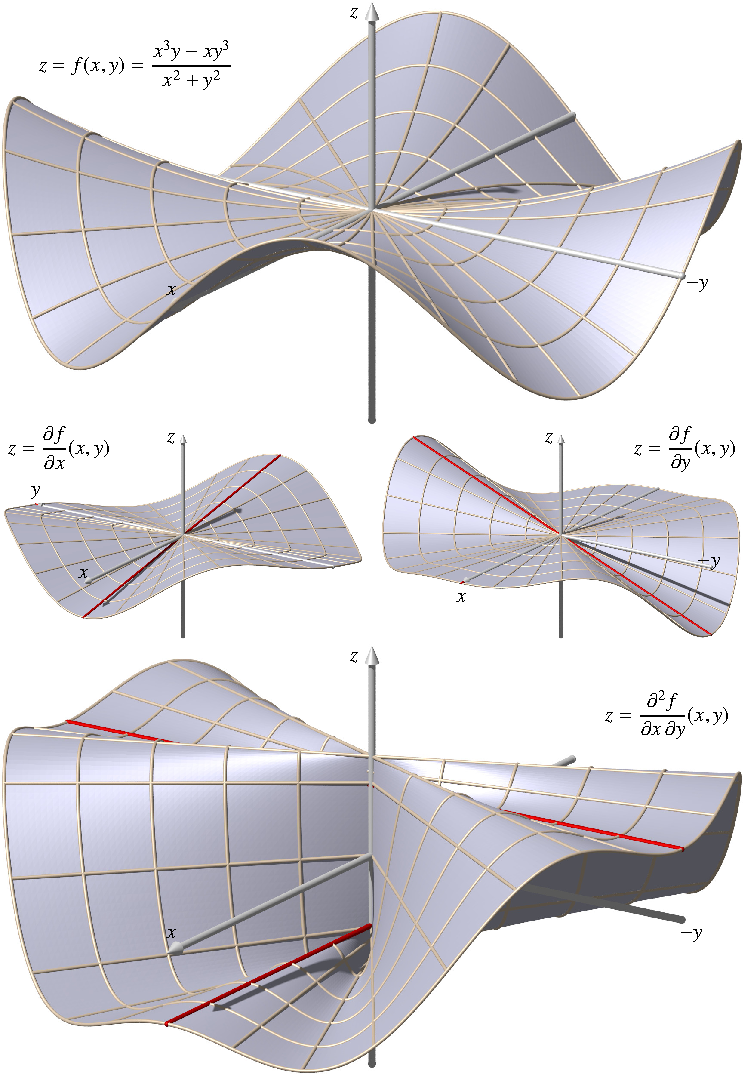
\includegraphics{chapters/010-fuvar/images/schwarz.pdf}
\caption{Gegenbeispiel~\ref{buch:fuvar:richtungsableitung:beispiel:schwarz}
zum Satz von Schwarz.
Oben der Graph der Funktion $f(x,y)$, in der Mitte die beiden 
ersten partiellen Ableitungen.
Die gemischten Ableitungen in der untersten Abbildung ist an der
Stelle $(x,y)=(0,0)$ nicht mehr stetig.
\label{buch:fuvar:richtungsableitung:fig:schwarz}}
\end{figure}
